\documentclass[12pt]{article}
\usepackage[utf8]{inputenc}
\usepackage[spanish]{babel}
\usepackage{graphicx}
\usepackage{mathpazo}
\usepackage{url}
\begin{document}
\title{Server}
\author{Rafael}

\maketitle

\section{Servidor} % (fold)
\label{sec:servidor}
El componente servidor cumple el papel de nodo central para la concentración de la información y notificación de cambios detectados en los módulos lego.
Adicionalmente, permite al usuario controlar de forma directa cada uno de los recursos existentes en los legos conectados a la aplicación, entendiéndose como recurso a alguno de los elementos que puede controlar como la ventana, las luces, el aire acondicionado, etc.

La Figura \ref{sec:servidor} muestra la arquitectura operacional de los componentes del sistema.
En ella pueden identificarse a los legos distribuidos en el ambiente interactuando a través de la interfaz bluetooth con el servidor.

\begin{figure}
\centering
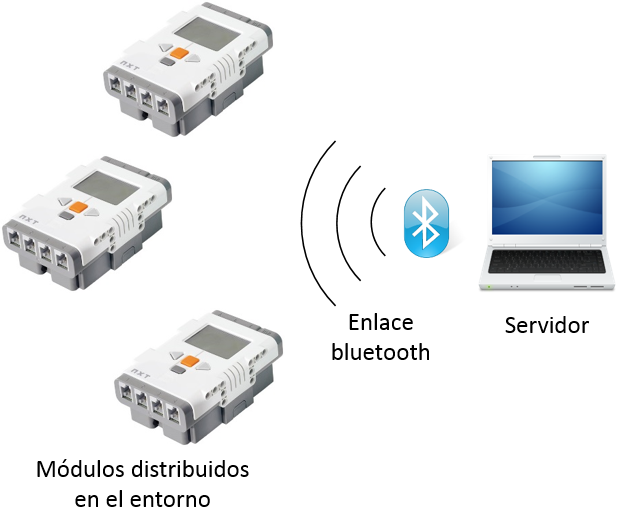
\includegraphics[width=\textwidth]{imagenes/arquitectura-operacional}
\caption[Arquitectura operacional]{Arquitectura operacional del sistema.}
\label{fig:arquitectura-operacional}
\end{figure}

Con el objetivo de alcanzar la funcionalidad previamente descrita, el servidor se ha diseñado considerando tres elementos principales: el motor de base de datos, la aplicación web y el motor de bluetooth.

La Figura \ref{fig:distribucion-elementos} muestra la distribución de los elementos del servidor y su interacción con el resto de participantes del sistema.
En dicha figura puede apreciarse cómo un usuario a través de un navegador web (incluso a través de un dispositivo móvil) podría interactuar con la aplicación web.

También, en la figura es posible detectar la interacción que el motor de bluetooth mantiene con los legos dispersos en el ambiente.
Asimismo, la figura muestra la vía de interacción entre el motor de base de datos y el software SGBD como tal.

\begin{figure}
\centering
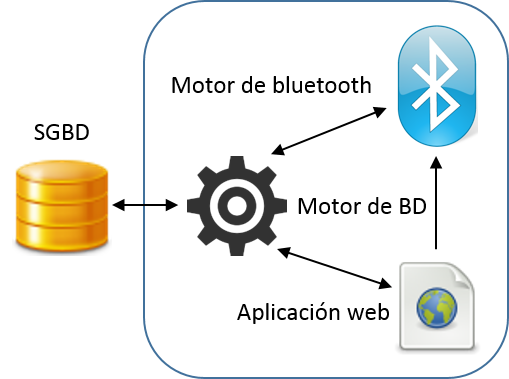
\includegraphics[width=\textwidth]{imagenes/distribucion-elementos}
\caption[Arquitectura operacional]{Interacción entre los elementos del servidor.}
\label{fig:distribucion-elementos}
\end{figure}

Es importante también destacar que inclusive los elementos mantienes mecanismos de interacción internos.
El motor bluetooth y la aplicación web consumen y generan datos a través del motor de la base de datos, mientras que la aplicación web únicamente solicita servicios al motor de bluetooth para realizar la manipulación directa de los recursos.
Las siguientes subsecciones describen a detalle cada uno de los componentes del servidor.

\subsection{Motor de base de datos} % (fold)
\label{ssub:motor_de_base_de_datos}
El motor de la base de datos funciona como la capa de acceso a los datos (Data Access Layer) de la aplicación.
Dentro de su funcionamiento se incluye la lógica básica para interactuar con el repositorio de almacenamiento, en este caso el SGBD\footnote{SGBD, Sistema Gestor de Base de Datos. URL: \url{http://es.wikipedia.org/wiki/Sistema_de_gestión_de_bases_de_datos}} MySQL, así como la definición de las tareas para dar de alta módulos en el sistema, establecimiento de horarios y obtención de datos para la generación de reportes.

La implementación técnica de este elemento fue desarrollada en la plataforma Java utilizando el framework de persistencia Hibernate\footnote{Hibernate ORM, Idiomatic persistence for Java and relational databases. URL: \url{http://hibernate.org/orm/}}. Dicho framework es un ORM\footnote{ORM, Object Relational Mapping. Puede obtenerse una descripción rápida en \url{http://es.wikipedia.org/wiki/Mapeo_objeto-relacional}} que permite traducir datos almacenados en tablas de una base de datos hacia objetos de la plataforma Java y viceversa.

Finalmente, es importante mencionar que este motor fue implementado de forma aislada, de tal manera que la aplicación web y el motor de bluetooth lo utilizan como biblioteca de dependencia.
De esta forma se omitió la  duplicación de código y se favoreció la el desarrollo del sistema por módulos.

\subsection{Aplicación web} % (fold)
\label{sub:aplicacion_web}
El objetivo principal de este elemento es proveer un medio para interacción directa con el usuario.
A través de la funcionalidad expuesta por la aplicación, es posible que el usuario agregue legos a la plataforma, manipule directamente cada uno de los recursos, establezca horarios de operación para los legos y realice la generación de reportes.

Como ha sido mencionado, la aplicación web consume la funcionalidad proporcionada por el motor de base de datos, canalizando las solicitudes de operación del usuario a los almacenes (tablas) correspondientes.

Asimismo, la aplicación web ofrece interacción con el motor de bluetooth en el momento en que el usuario indique la manipulación directa de los recursos, así como el establecimiento de horarios para su utilización.


Técnicamente, la aplicación web define una serie de servicios web RESTful\footnote{REST, Representational State Transfer. Servicios web basados en los estados disponibles en el estándar HTTP. Puede obtenerse una descripción rápida en: \url{http://es.wikipedia.org/wiki/Representational_State_Transfer}} que son consumidos por las páginas web desplegadas en el navegador del usuario. Estos servicios son creados utilizando la librería Jersey\footnote{Jersey, RESTful Web Services in Java. URL: \url{https://jersey.java.net/}} y son publicados como una aplicación web a través del servidor de aplicaciones Glassfish.

Debido a que la funcionalidad de la aplicación es expuesta como una API a través de servicios web, es posible la generación de nuevas aplicaciones que al consumir los servicios tengan una funcionalidad equivalente.
% subsection aplicación_web (end)

\subsection{Motor bluetooth} % (fold)
\label{sub:motor_bluetooth}
El motor de bluetooth es el corazón del sistema para realizar la interacción con el conjunto de legos dispersos en el ambiente.
Debido a la naturaleza de la tecnología bluetooth implementada en los legos, se requiere que exista un maestro entre los dispositivos interconectados, el cual es el único que puede iniciar la comunicación.


Por la razón anterior, se ha elegido a una computadora como el elemento externo para que actúe como maestro y coordine la comunicación, recolección de datos y notificación de eventos entre los dispositivos lego conectados al sistema.

El motor bluetooth se encuentra en ejecución permanente realizando un conjunto de tareas, mostradas en la Figura \ref{fig:etapas-operacion-servidor}, ejecutadas en un ciclo infinito en el mismo orden en el que a continuación se describen.

\begin{figure}
\centering
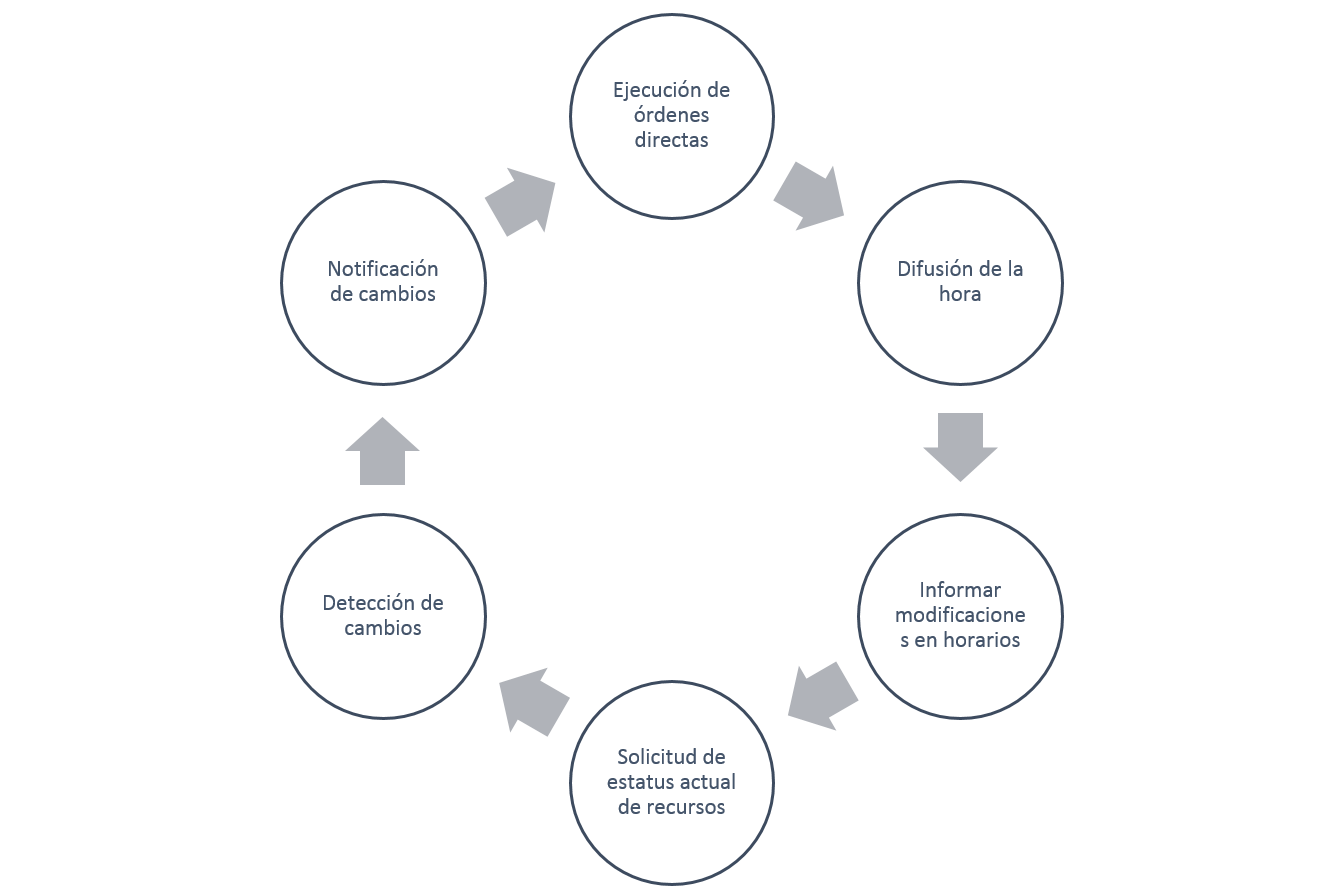
\includegraphics[width=\textwidth]{imagenes/etapas-operacion-servidor}
\caption[Etapas en la operación del servidor bluetooth]{Etapas en la operación del servidor bluetooth.}
\label{fig:etapas-operacion-servidor}
\end{figure}

\begin{itemize}
	\item \textbf{Ejecución de órdenes directas}: Es posible que el usuario que utilice la aplicación web indique el encendido o apagado de alguno de los recursos administrados por los legos.
	Por esta razón, el motor bluetooth permite la recepción de dichas órdenes y las canaliza directamente a los legos.

	Es importante hacer notar que la aplicación web no instruye a legos para hacer cambios en el estado de los recursos, sino que solicita al motor de bluetooth su intervención para la ejecución de esta labor.
	Las solicitudes de ejecución de órdenes son puestas en una cola y dispuestas para su ejecución en esta etapa.

	\item \textbf{Difusión de la hora}: Los kits legos utilizados en esta implementación carecen de un reloj interno, por lo que se requiere la difusión de la hora del sistema entre los módulos participantes.
	La hora del sistema es tomada del servidor y se envía de forma periódica hacia los legos.

	Gracias a que los legos son conscientes de la hora del sistema, es posible que puedan definir horarios de operación.

	\item \textbf{Informar modificaciones en la configuración de  horarios}: Es posible utilizar la aplicación web para modificar los distintos horarios de operación de los recursos. 

	Al igual que la solicitud de ejecución de órdenes directas, las solicitudes de cambios en los horarios son puestas en una cola y notificados al lego indicado en cuanto se alcance este paso de la operación.

	\item \textbf{Solicitud del estatus actual de los recursos}: En esta etapa, el motor de bluetooth realiza la solicitud del estatus de los recursos administrados por cada lego del sistema.
	A través de una solicitud de servicio al motor de base de datos, el motor de bluetooth es capaz de identificar cuáles son los recursos manipulados por cada lego, solicitando únicamente la información de los recursos pertinentes. 

	Gracias a esta labor, el sistema es capaz de generar una matriz con el estado global actual del sistema.

	\item \textbf{Detección de cambios (eventos) en el sistema}: En esta etapa, el motor de bluetooth realiza una comparación entre la matriz con el estado global actual del sistema y la matriz obtenida en la iteración anterior.

	El resultado de este proceso comparativo es identificado como u conjunto de cambios o eventos ocurridos en el sistema y se almacenan a través de la funcionalidad ofrecida por el motor de base de datos para la generación de reportes.

	\item \textbf{Notificación de cambios (eventos)}: Una vez que los cambios han sido detectados, el motor de bluetooth requiere notificar, a manera de broadcast lógico, a los componentes del sistema acerca de los nuevos eventos que definen un nuevo estado en el ambiente de la aplicación.
	De esta manera, cada uno de los legos conoce lo que sucede a su alrededor.

\end{itemize}


De forma técnica, la implementación del motor de bluetooth concentró su complejidad en los aspectos de comunicación definidos por el sistema operativo de los legos.

Utilizando la librería jssc\footnote{jssc, Java Simple Serial Connector \url{https://code.google.com/p/java-simple-serial-connector/}} en el lado del servidor, se utilizó la noción de puerto serial virtual existente en el sistema operativo (en este caso Windows 7); de esta forma la implementación del mecanismo de comunicación es agnóstica a los detalles físicos y técnicos inherentes a la comunicación bluetooth.
Esto se refiere a que en primera instancia los dispositivos deben ser emparejados con el servidor a nivel sistema operativo.
Posteriormente, la aplicación tiene acceso a un puerto en el que ya existe un destinatario de la comunicación, eliminando los procesos de búsqueda de dispositivos bluetooth, identificación de direcciones MAC, etc.


La implementación en los legos fue realizada utilizando una librería especial para la comunicación bluetooth\footnote{NXT to NXT communication, using NXC programs, \url{http://www.alfonsomartone.itb.it/yepuji.html}}. 
Esta librería cuenta con soporte para la sincronización del envío y recepción de mensajes, así como tareas de verificación del estatus de la conexión de forma permanente.

De esta forma, fue posible obtener un mecanismo de interacción fiable y robusto, según las pruebas realizadas, entre el servidor y los legos.

Es importante mencionar que en la implementación se obtuvo un mecanismo de comunicación que a alto nivel se comporta como full-dúplex pero que bajo nivel en realidad es half-dúplex.

Adicionalmente, se destaca que aunque solamente sea necesario enviar información del servidor (master) hacia los legos (esclavos), estos últimos siempre responden con al menos un estatus de la recepción de los datos; esto significa que por cada interacción a alto nivel entre el servidor y los legos, en realidad existen dos eventos de comunicación en la infraestructura de comunicación inalámbrica.

Finalmente, es importante describir que la implementación del motor bluetooth también incluyo la definición y despliegue de un par de servicios web. 
Estos servicios fueron publicados para tener un mecanismo que le permita al motor bluetooth recibir solicitudes de manipulación directa de los recursos y establecimiento de horarios de operación.
Gracias a esto la aplicación web puede solicitar al motor bluetooth la ejecución de estas tareas especiales.

% subsection motor_bluetooth (end)


% section servidor (end)

\end{document}